% !TEX root = ../proj_report_outline.tex

\chapter{Three-way Tensors and Bilinear Products}\label{C:tens}

In order to represent functions of two arguments with neural networks, three-way tensors are 
unavoidable. In this chapter we discuss the vector-tensor-vector bilinear product and assess its
suitability, both theoretically and empirically, to be used inside a neural network,

This product admits a surprising
number of interpretations including theorem~\ref{thm:xor} -- that it allows us to operate on a
pairwise exclusive-or of features. This is a powerful result which shows that admitting tensors
into neural networks can solve the exclusive-or problem without any hidden units. Further, we
demonstrate the expressive power of the tensor by showing that a polynomially sized network with a
single tensor product is capable of expressing a class of functions which standard two layer networks
can not approximate accurately without exponential size.

The downside of these tensor products is the storage requirements. We investigate methods for
decomposing tensors into products of smaller objects. Finally we conduct experiments to show that
learning the coefficients of a decomposed tensor can be done in situ with gradient descent. We attempt
to investigate the tradeoff between the complexity of the decomposition and the expressivity of the
product and find that it scales as expected.

\section{Definitions}
Formally, we refer to a multi-dimensional array which requires \(n\) indices to address a single
(scalar) element as a \(n\)-way tensor and occasionally refer to \(n\) as the number of dimensions of
the tensor. In this sense a matrix is a two-way tensor and a vector
a one-way tensor, although we will use their usual names for clarity. Notationally, we attempt to
stick to the notation used in \autocite{Kolda2009} deviating only where it would become unwieldy.
We denote tensors with three or more dimensions with single calligraphic boldface letters such
as \(\tensor{W}\). Matrices and vectors will be denoted with upper and lower case boldface letters
while scalars will be standard lower case letters. We will often need to address particular
substructures of tensors. This is analogous to pulling out individual rows or columns of a matrix.
To perform this we fix some of the indices to specific values and allow the remaining indices to vary
across their range. We denote by \(\midbullet\) the indices allowed to vary, the rest will be provided
with a specific value. For example, \(\mat{A}_{i \midbullet}\) would denote the \(i\)-th row of the
matrix \(\mat{A}\).
For three-way tensors we refer to the vector elements produced by fixing two indices as 
\emph{threads}. It is also possible to form matrices by fixing only one index -- we refer to these
as \emph{slices}. Table~\ref{tab:notation} provides examples of the possibilities.

\begin{table}
\centering
\begin{tabu} to 0.5\linewidth {|r|l|}
\hline 
\textit{Description} & \textit{Example} \\
\hline
scalar & \(a\) \\
vector & \(\vec{b}\) \\
matrix & \(\mat{C}\) \\
higher order tensor & \(\tensor{D}\) \\
element of vector (scalar) & \(b_i\) \\
element of matrix (scalar) & \(C_{ij}\) \\
element of 3-tensor (scalar) & \(D_{ijk}\) \\
row of matrix (vector) & \(\vec{C}_{i\midbullet}\) \\
column of matrix (vector) & \(\vec{C}_{\midbullet i}\)\\
\textit{fiber} of 3-tensor (vector) & \(\vec{D}_{\midbullet jk}\)\\
\textit{slice} of 3-tensor (matrix) & \(\mat{D}_{\midbullet\midbullet k}\)\\
\hline
\end{tabu}
\caption{Example of notation for tensors.}
\label{tab:notation}
\end{table}

When dealing with tensor-tensor products, it is important to be precise as there are often
a number of possible permutations of indices that would lead to a valid operation. The downside of
this is that it leads to unwieldy notation. Fortunately, we are only concerned with a a couple of
special cases. In particular, we need to multiply a three-tensors by vectors and a matrices by
vectors. Matrix-vector multiplication consists of taking the dot product of the vector with
each row of the matrix. For example, with a matrix \(\mat{A} \in \mathbb{R}^{m \times n}\) and a
vector \(\vec{x} \in \mathbb{R}^n\), if \(\vec{y} = \mat{A}\vec{x}\) (with \(\vec{y}\) necessarily
in \(\mathbb{R}^m\)), then
\begin{equation}\label{eq:matmul}
	y_i = \sum_j^n A_{ij} x_j
		= \langle \vec{A}_i, \vec{x}\rangle
\end{equation} where \(\langle \cdot, \cdot \rangle\) denotes the inner (dot) product. This can be viewed
as taking all of the vectors formed by fixing the first index of \(\mat{A}\) while allowing the second
to vary and computing their inner product with \(\vec{x}\). To perform the same operation using the
columns of \(\mat{A}\) we need to fix the second index, the would typically be done by exchanging the
order: \(\tran{\vec{x}}\mat{A}\). This kind of operation is sometimes referred to as a
\emph{contractive} product, especially in the physical sciences \autocite{Orus2014}. This name
arises because we form the output by joining a shared dimension (by element-wise multiplication) and
contracting it with a sum.

We can generalise the operation to tensors: choose an index over which to perform the product,
collect every thread formed by fixing all but that one index and compute their inner product with the
given vector. If the tensor has \(n\) indices, the result will have \(n-1\). A three tensor is in
this way reduced to a matrix. Kolda and Bader introduce the operator
 \(\;\cdot \bar{\times}_i \cdot\;\)
for this, where \(i\) represents the index to vary \autocite{Kolda2009}. For the bilinear forms
we are concerned with, this leads to the following notation:
\begin{align}
	\vec{z} &= \tensor{W} \;\bar{\times}_1\; \vec{x}\; \bar{\times}_2\; \vec{y} .
	\label{eq:bilinearkolda}
\end{align}

\begin{figure}
	\centering
	\begin{subfigure}[t]{0.45\textwidth}
	\centering
	\begin{tikzpicture}
		\draw (0,0) node {} -- (-1,0);
	\end{tikzpicture}
	\caption{Vector \(\vec{a}\in\mathbb{R}^{n_1}\)}\label{fig:tnd:vec}
	\end{subfigure} ~
	\begin{subfigure}[t]{0.45\textwidth}
	\centering
	\begin{tikzpicture}
		\draw (1,0) -- (0,0) node {} -- (-1,0);
	\end{tikzpicture}
	\caption{Matrix \(\mat{B}\in\mathbb{R}^{n_1 \times n_2}\)}\label{fig:tnd:mat}
	\end{subfigure} \\
	
	\begin{subfigure}[t]{0.5\textwidth}
	\centering
	\begin{tikzpicture}
		\draw (0,0) node {}
			\foreach \x in {0,90,180}
			{
				(\x:1) -- (0,0)
			};
	\end{tikzpicture}
	\caption{Three-way tensor 
		\(\tensor{C}\in\mathbb{R}^{n_1\times n_2\times n_3}\)}\label{fig:tnd:3ten}
	\end{subfigure}
	\caption{Example tensor network diagrams.}
	\label{fig:tnegs}
\end{figure}

When \(\tensor{W}\) is a three-way tensor, we prefer a more compact notation
\begin{equation}\label{eq:bilintensor}
	\vec{z} = \tran{\vec{x}}\tensor{W}\vec{y}.
\end{equation} This loses none of the precision of the more verbose notation provided we make clear
that we intend \(\vec{x}\) to operate along the first dimension of the tensor and \(\vec{y}\) the
third such that \((\tran{\vec{x}}\tensor{W})\vec{y}\) exactly corresponds with 
equation~\eqref{eq:bilinearkolda}. With either notation, for a tensor 
\(\tensor{W} \in \mathbb{R}^{n_1 \times n_2 \times n_3}\), we must have that 
\(\vec{x}\in \mathbb{R}^{n_1}\), \(\vec{y} \in \mathbb{R}^{n_3}\) and the result 
\(\vec{z}\in\mathbb{R}^{n_2}\).

An intuitive way to illustrate these ideas is using Tensor Network Diagrams
\autocite{Cichocki2016, Orus2014}. In these diagrams, each object is represented
as a circle, with each free `arm' representing an index used to address elements.
A vector therefore has one free arm, a matrix two and so on. Scalars will have
no arms. Figure~\ref{fig:tnegs} provides examples for these simple objects. 

Where these diagrams are especially useful is for representing contractive products
where we sum over the range of a shared index. We represent this by joining the
respective arms. As an example, a matrix-vector product \(\vec{y} = \mat{Ax}\)
has such a contraction: \(y_{i} = \sum_{j}A_{ij}x_{j}\). This is shown in
figure~\ref{fig:tnmatvec} -- it is clear that there is only a single free arm, so the
result is a vector as it should be. Figure~\ref{fig:tnprods} shows some examples
of these kinds of products.

\begin{figure}
	\centering
	\begin{subfigure}[t]{0.45\textwidth}
		\centering
		\begin{tikzpicture}
			\draw
				(1,0) node (A){} -- (0,0) node(y) {} 
				-- (-1,0);
			\node[below=1em of A, fill=none, draw=none, anchor=mid] {\(\mat{A}\)};
			\node[below=1em of y, fill=none, draw=none, anchor=mid] {\(\vec{y}\)};
		\end{tikzpicture}
		\caption{Matrix-vector product \(\mat{A}\vec{y}\), one free arm indicates
		 the result is a vector.}
		 \label{fig:tnmatvec}
	\end{subfigure} ~
	\begin{subfigure}[t]{0.45\textwidth}
		\centering
		\begin{tikzpicture}
			\draw
				(-1,0) node(x){} -- 
				(0,0) node(A) {} --
				(1,0) node(y){};
			\node[below=1em of x, fill=none, draw=none, anchor=mid] {\(\tran{\vec{x}}\)};
			\node[below=1em of A, fill=none, draw=none, anchor=mid] {\(\mat{A}\)};
			\node[below=1em of y, fill=none, draw=none, anchor=mid] {\(\vec{y}\)};
		\end{tikzpicture}
		\caption{Vector-matrix-vector bilinear form \(\tran{\vec{x}}\mat{A}
				 \vec{y}\). No free arms so the result is a scalar.}
	\end{subfigure}\\
	\begin{subfigure}[t]{0.45\textwidth}
		\centering
		\begin{tikzpicture}
			\draw (0,0) node(W) {}
				(180:1) -- node[above, fill=none, draw=none]{\(n_1\)} (0,0)
				(0:1) node(y){} -- node[above, fill=none, draw=none]{\(n_3\)} (0,0)
				(90:1) -- node[above right=1em, fill=none, draw=none]{\(n_2\)} (0,0);
			\node[below=1em of W, fill=none, draw=none, anchor=mid] {\(\tensor{W}\)};
			\node[below=1em of y, fill=none, draw=none, anchor=mid] {\(\vec{y}\)};
		\end{tikzpicture}
		\caption{Tensor-vector product producing a matrix.}
	\end{subfigure} ~
	\begin{subfigure}[t]{0.45\textwidth}
		\centering
		\begin{tikzpicture}
			\draw (0,0) node(W) {}
				(180:1) node(x){} -- node[above, fill=none, draw=none]{\(n_1\)} (0,0)
				(0:1) node(y){} --node[above, fill=none, draw=none]{\(n_3\)}  (0,0)
				(90:1) -- node[above right=1em, fill=none, draw=none]{\(n_2\)} (0,0);
			\node[below=1em of x, fill=none, draw=none, anchor=mid] {\(\tran{\vec{x}}\)};
			\node[below=1em of W, fill=none, draw=none, anchor=mid] {\(\tensor{W}\)};
			\node[below=1em of y, fill=none, draw=none, anchor=mid] {\(\vec{y}\)};
		\end{tikzpicture}
		\caption{Vector-tensor-vector product produces a vector.}
		\label{fig:vanillabilintnd}
	\end{subfigure}
	\caption{Various products expressed as Tensor Network Diagrams.}
	\label{fig:tnprods}
\end{figure}

\section{Bilinear Products}
There are several ways to describe the operation performed by the bilinear products we are
concerned with. These correspond to different interpretations of the results. The following
interpretations provide insight both into what is actually being calculated and how the product might
be applicable to a neural network setting. In all of the below we use the above definitions of
\(\vec{x}, \vec{y}, \vec{z}\) and \(\tensor{W}\).

\subsection{Interpretations}\label{sec:tensorinterps}
\subsubsection{Stacked bilinear forms}
If we consider the expression for a single element of \(\vec{z}\), we get
\begin{equation} \label{eq:singlezsum}
	z_j = \sum_i^{n_1} \sum_k^{n_3} W_{ijk} x_i y_k
\end{equation} as expected. We can re-write this in terms of the slices of \(\tensor{W}\):
\begin{equation}\label{eq:singlezslice}
	z_j = \tran{\vec{x}}\tensor{W}_{\cdot j \cdot}\vec{y}
\end{equation} which reveals the motivation behind the notation in equation~\eqref{eq:bilintensor}.
It also reveals that each element of \(\vec{z}\) is itself linear in \(\vec{x}\) or \(\vec{y}\) if
the other is held constant.

This provides an interpretation
in terms of similarities. If we consider the standard dot product of two vectors 
\(\vec{a}\) and
\(\vec{b}\) of size \(m\): 
\begin{equation}
\langle\vec{a}, \vec{b}\rangle = 
\vec{a}^\mathsf{T}\vec{b}
= \sum_{i=1}^ma_ib_i
 = {\cos\theta}{\cdot||\vec{a}||_2\cdot||\vec{b}||_2} 
\end{equation} where
\(\theta\) is the angle in the angle between the vectors. If the product
is positive, the two vectors are pointing in a similar direction and if it is negative they
are in opposite directions. If it is exactly zero, they must be orthogonal. The dot product
therefore provides us with a notion of the similarity between two vectors.
Indeed if we normalise the vectors by dividing each component by their \(l_2\) norm we
recover exactly the widely used cosine similarity, common in information retrieval 
\autocite{Singhal2001, Tan2006} . Note that
we can generalise this idea by inserting a matrix of (potentially learned)
weights \(\mat{U}\) which enables us
to define general scalar bilinear forms
\begin{equation}
	\langle\vec{a}, \mat{U}\vec{b}\rangle = \langle\vec{a}^\mathsf{T}\mat{U}, \vec{b}\rangle
	= \vec{a}^\mathsf{T}\mat{U}\vec{b}.
\end{equation}

In a bilinear tensor product, each component of the result takes this form.
We can therefore think of the
product as computing a series of distinct similarity measures between the two input
vectors. With this in mind the obvious question is: what is the role of the matrix? The first
thing to note is that inserting a matrix into the inner product allows the two vectors to be
of different dimension. We also observe that a matrix-vector multiplication consists of
taking the dot product of the vector with each row or column of the matrix. Given our current
interpretation of the dot product as an un-normalised similarity measure, we can also
interpret a matrix-vector multiplication as computing the similarity of the vector with each
row or column of the matrix. 

We can then think of the rows of the matrix \(\mat{U}\) in the
above as containing patterns to look for in the \(\vec{b}\) vector and the columns to
contain patterns to test for in the \(\vec{a}\) vector. If we consider the vectors 
\(\vec{a}\) and \(\vec{b}\) to come from different feature spaces, the matrix \(\mat{U}\)
provides a conversion between them allowing us to directly compare the two. We can then
interpret each coordinate of the result of the bilinear tensor product as being an
independent similarity measure based on different interpretations of the underlying
feature space. In this sense, where a matrix multiplication looks for patterns in a single input
space, a bilinear product looks for \emph{joint} patterns in the combined input spaces of
\(\vec{x}\) and \(\vec{y}\). This becomes clear if we write out each element of the result
vector
\begin{equation} \label{eq:features}
	\vec{z} = \begin{bmatrix}
		\tran{\vec{x}}\mat{W}_{\midbullet 1 \midbullet}\vec{y} \\
		\tran{\vec{x}}\mat{W}_{\midbullet 2 \midbullet}\vec{y} \\
		\vdots \\
		\tran{\vec{x}}\mat{W}_{\midbullet n_2 \midbullet}\vec{y}
	\end{bmatrix}
	= \begin{bmatrix}
		\langle\vec{x}, \mat{W}_{\midbullet 1 \midbullet} \vec{y}\rangle \\
		\langle\vec{x}, \mat{W}_{\midbullet 2 \midbullet} \vec{y}\rangle \\
		\vdots \\
		\langle\vec{x}, \mat{W}_{\midbullet n_2 \midbullet} \vec{y}\rangle
	\end{bmatrix}
	 = \begin{bmatrix}
	 	\cos \theta_1 \cdot ||\vec{x}||_2 \cdot ||\mat{W}_{\midbullet 1 \midbullet}\vec{y}||_2 \\
	 	\cos \theta_2 \cdot ||\vec{x}||_2 \cdot ||\mat{W}_{\midbullet 2 \midbullet}\vec{y}||_2 \\
		\vdots \\
	 	\cos \theta_{n_2} \cdot ||\vec{x}||_2 \cdot ||\mat{W}_{\midbullet n_2 \midbullet}\vec{y}||_2 \\
	 \end{bmatrix}.
\end{equation}


\subsubsection{Choosing a matrix}
Following on from the above discussion we claim that for each coordinate of the output we are
computing a \emph{similarity vector} which we compare to the remaining input to generate a
scalar value. If we consider all coordinates at once, we see that this amounts to having
one input choose a matrix, which we then multiply by the remaining input vector. We have
refrained from making these points in terms of the specific vectors referenced above to make
the point that the operation is completely symmetrical. While it aids interpretation to think
of one vector choosing a matrix for the other vector, we can always achieve the same
intuition after switching the vectors, give or take some transposes.

This interpretation is very clear from the expression of the product in
equation~\eqref{eq:bilinearkolda}. Simply by inserting parentheses we observe that we are
first generating a matrix in a way somehow dependent on the first input and multiplying
the second input by that matrix. In this sense we allow one input to choose patterns to look for
in the other input.

This intuition of choosing a matrix is suggested in \autocite{Sutskever2013} in the
context language modelling with RNNs. It is suggested that allowing the current input
character to choose the hidden-to-hidden weights matrix should confer benefits. 
This intuition (and the factorisation of the implicit tensor) was put to use earlier in
of Conditional Restricted Boltzmann Machines \autocite{Taylor} which actively seek to model the
conditional dependencies between two types of input.

Although this provides a powerful insight into the bilinear product, it is worth reinforcing that
the product is entirely symmetrical. We can not think purely about it as \(\vec{x}\) choosing a matrix
for \(\vec{y}\) as the converse is equally true.

\subsubsection{Tensor as an independent basis}
Extending the above to try and capture the symmetry of the operation, we introduce
the notion that the coefficients of the tensor represent a basis in which to compare the
two inputs, independent of both of them. This idea is mentioned in
 \autocite{Tenenbaum2000} which considered the problem of data that can be described by two
independent factors.
The tensor then contains a basis which characterises the interaction by which the factors
in the input vectors combine to create an output observation.

This is a somewhat abstract interpretation -- to attempt to create a more concrete
 intuition
consider the case when both vectors have a single element set to \(1\) and the remainder
\(0\). In this case the first tensor-vector product corresponds to taking a slice of the
tensor, resulting in a matrix. The final matrix-vector product corresponds to picking a
row or column of the matrix. Consequently the whole operation is precisely looking up
a fibre of the tensor. To generalise from such a ``one-hot'' encoding of the inputs
to vectors of real coefficients, we simply replace the idea of a
\emph{lookup} with that of a \emph{linear combination}. The vectors then represent the coefficients
of weighted sums; first over slices and then over rows or columns. The final product is then a
distinct representation of both vectors in terms of the independent basis expressed by the tensor.

\subsubsection{Operation on the outer product}
Perhaps the most powerful interpretation of the product is achieved by observing that it is
a linear operation on pairwise products of inputs.
This interpretation is essential for understanding the expressive
power of the operation as it gives rise to an obvious XOR-like behaviour. It also serves
as a useful reminder that a bilinear form is linear in each input only when the other
is held constant -- when both are allowed to vary we can represent complex non-linear
relations.
A way to approach this interpretation arises from a method of implementing the bilinear 
product in terms of straightforward matrix operations.

To discuss
this we need to introduce the \emph{matricisation} of a tensor. Intuitively this
operation is a way of \emph{unfolding} or \emph{flattening} a tensor into a matrix,
preserving its elements. Specifically the mode-\(n\)
matricisation of a tensor is defined as an operation which takes all mode-\(n\) fibres
of the tensor and places them as columns to create a matrix. We denote an mode-\(n\)
matricisation of a tensor \(\tensor{W}\) as \(\matr_n(\tensor{W})\). While the operation is
fairly straightforward, describing the exact permutation of the indices is awkard -- 
for a robust treatment of the general case (and the source of the above definition) see
\autocite{Kolda2009}. 

As an example consider the three-way tensor \(\tensor{X} \in \mathbb{R}^{2 \times 3 \times 4}\)
with slices
\begin{align} \label{eq:slicies}
	\mat{X}_{1 \midbullet \midbullet} &= \begin{bmatrix}
		a & d & g & j \\
		b & e & h & k \\
		c & f & i & l \\
	\end{bmatrix} \\
	\mat{X}_{2 \midbullet \midbullet} &= \begin{bmatrix}
		m & p & s & v \\
		n & q & t & w \\
		o & r & u & x \\
	\end{bmatrix}.
\end{align} To construct \(\matr_2(\tensor{X})\) we fix the first and third indices and place the
resulting threads as columns of a new matrix. Fixing the first index corresponds to choosing one of
the slices presented above while fixing the third amounts to choosing a column of one of the slices.
The result is:
\begin{equation}\label{eq:matricisedeg}
	\matr_2(\tensor{X}) = \begin{bmatrix}
		a & d & g & j & m & p & s & v \\
		b & e & h & k & n & q & t & w \\
		c & f & i & l & o & r & u & x
	\end{bmatrix}.
\end{equation}

Although this notion captures and generalises the vectorisation operator often
encountered in linear algebra, we retain the classical \(\vect\) operator for clarity.
This flattens a matrix into a vector by stacking its columns. For some matrix \(\mat{A}\) with
\(n\) columns:
\begin{equation}\label{eq:vec}
	\vect(\mat{A}) = \begin{bmatrix}
		\vec{A}_{\midbullet 1}\\
		\vec{A}_{\midbullet 2}\\
		\vdots\\
		\vec{A}_{\midbullet n}
	\end{bmatrix}.
\end{equation}

For our purposes is is sufficient to note that a 
mode-2 matricisation of a
three-way tensor \(\tensor{W} \in \mathbb{R}^{n_1\times n_2\times n_3}\) must have shape
\(n_2 \times n_1n_3\). The following lemma helps us describe the components of this matricisation.

\begin{lem}[Matricisation/vectorisation]
The \(j\)-th row of the mode-2 matricisation of the three-way tensor \(\tensor{W}\)
is equivalent to the vectorisation of the transpose of the slice formed by fixing the second index 
at \(j\):
\begin{equation}\label{eq:matlemstatement}
	\matr_2 (\tensor{W})_{j \midbullet} = \vect(\tran{\mat{W}_{\midbullet j \midbullet}}).
\end{equation}
\label{lem:matricise}
\end{lem}
\begin{proof}
By the above definition of the vectorisation operator, each index \((i, k)\) in some matrix
\(\mat{U} \in \mathbb{R}^{n_1\times n_3}\) maps to element \(i + (k-1)n_1\) in
\(\vect(\mat{U})\). By the definition of the mode-2 matricisation we would expect to
find tensor element \(W_{ijk}\) at index \((j, i + (k-1)n_3)\). Hence if we fix \(j\), we have
precisely the vectorisation of the \(j\)-th slice of the tensor.

The indices into \(\matr_2(\tensor{W})\) can be though of as arising from the following construction.
First fix all indices to 1. Construct a column by sweeping the second index, \(j\),
through its full range. Then increment the first index \(i\) and repeat the procedure, placing
the generated columns with index \(i\). Only when \(i\) has swept through its full range
increment the final index \(k\) and repeat the procedure. The generated columns should then be
at positions \(i + (k-1)n_1\).
\end{proof}

To understand the lemma it helps to consider an example. Using the \(2 \times 3 \times 4\)
tensor \(\tensor{X}\) defined
in equation~\eqref{eq:slicies}, fixing the second index to \(2\) gives a \(4 \times 2\) 
transposed slice:
\begin{equation}\label{eq:mode2slice}
	\tran{\mat{X}_{\midbullet 2 \midbullet}} = \begin{bmatrix}
		b & n \\
		e & q \\
		h & t \\
		k & w
	\end{bmatrix}.
\end{equation} Vectorising this matrix takes each column and stacks them, giving
\begin{equation}\label{eq:veceg}
	\vect(\tran{\mat{X}_{\midbullet 2 \midbullet}}) = \begin{bmatrix}
		b \\
		e \\
		h \\
		k \\
		n \\
		q \\
		t \\
		w
	\end{bmatrix}
\end{equation} which is precisely row two in equation~\eqref{eq:matricisedeg}.

These flattenings are important as they allow us to
implement many operations involving tensors in terms of a small number of larger matrix
operations when compared to the naive approach.

\begin{lem}[Matricised product]\label{lem:outerprod}
For a tensor \(\tensor{W}\) and vectors \(\vec{x}, \vec{y}\) as above,
we can describe the product \(\vec{z} = \tran{\vec{x}}\tensor{W}\vec{y}\) in terms of the
mode-2 matricisation of \(\tensor{W}\) as 
follows:
\begin{align}
	\vec{z} = \matr_2(\tensor{W})\mathrm{vec}\left[\vec{y}\tran{\vec{x}}\right]
	\label{eq:bilinearouter}
\end{align}
\end{lem}

\begin{proof}
To
prove this we can compare the expressions for a single element of the result.
An element \(z_j\) from equation~\eqref{eq:bilinearouter}
is formed as the inner product of the \(j\)-th
row of the flattened tensor and the vectorised outer product of the inputs. By 
lemma~\ref{lem:matricise}:
\begin{equation}
	z_j = 
	\sum_{s=1}^{n_1n_3} \left(\matr(\tensor{W})\right)_{js} \cdot
	\left( \vect\left[\vec{y}\tran{\vec{x}}\right]\right)_s
\end{equation}
We replace the sum over \(s\) with a sum over two
indices, \(i\) and \(k\), and using them to appropriately re-index the flattenings 
as described in lemma~\ref{lem:matricise} we 
derive
\begin{align}
	z_j &= \sum_{i=1}^{n_1}\sum_{k=1}^{n_3} W_{ijk} x_i y_k \\
		&= \tran{\vec{x}}\mat{W}_{\midbullet j \midbullet}\vec{y}
\end{align}

\end{proof}


Therefore to understand the bilinear product it helps to understand the matrix 
\(\vec{y}\vec{x}^\mathsf{T}\). This matrix takes the following form:
\begin{equation}\label{eq:outer}
	\vec{y}\tran{\vec{x}} = \begin{bmatrix}
		x_1y_1 & \ldots & x_{n_1}y_1 \\
		\vdots & \ddots & \vdots \\
		x_1y_{n_3} & \ldots & x_{n_1}y_{n_3}
	\end{bmatrix}
\end{equation} which contains all possible products of pairs of elements, one from each vector. 
This captures some interesting interactions.

\begin{thm} [Bilinear exclusive-or] \label{thm:xor}
Bilinear tensor products operate on the pair-wise exclusive-or of the
signs of the inputs.
\end{thm}
\begin{proof}
Consider the sign of a scalar product
\(c = a\cdot b\). If one of the operands \(a\) or \(b\) is positive and the other negative,
then the sign of \(c\) is negative. If both are positive or both are negative, then the
result is positive. This captures precisely the ``one or the other but not both'' structure
of the exclusive-or operation.

By lemma~\ref{lem:outerprod} a bilinear product can be viewed as a matrix operation on the flattened
outer product of the two inputs. As each element in the outer product is the product of two scalars,
the signs have an exclusive-or structure.
\end{proof}

\begin{cor}[Bilinear conjunctions]\label{cor:and}
If the inputs are binary, bilinear products operate on pair-wise conjunctions of the inputs.
\end{cor}
\begin{proof}
If \(a, b \in \{0, 1\}\), then \(a \cdot b = 1\) if and only if both \(a\) and \(b\) are \(1\). If
either or both are \(0\) then their product must be zero. Following the same structure as the proof
of theorem~\ref{thm:xor}, for binary inputs we must have this conjunctive relationship.
\end{proof}

\subsubsection{Implications}
%\paragraph{Higher level features}
Firstly, this captures the notion that the bilinear tensor product operates implicitly on higher
level features, constructed by combining both inputs. This indicates that it is capable of capturing
complex binary relationships based on correlations between both inputs. This allows it
to model a rich class of binary relations between \(\vec{x}\) and \(\vec{y}\).

%\paragraph{XOR}
Secondly this suggests considering
the case where both inputs are the same: \(\vec{z} = \tran{\vec{x}}\tensor{W}\vec{x}\). Replacing
bilinear forms with quadratic forms may invalidate some of the similarity based interpretations,
but it also provides an interesting building block for feed-forward networks. As an example,
note that a plain perceptron has been long known to be incapable of learning the exclusive-or
mapping \autocite{Minsky1969} -- a neural network to solve the problem requires either a hidden layer
or an additional input feature (specifically the conjunction of the inputs) \autocite{Rumelhart1986}.
By corollary~\ref{cor:and} this quadratic tensor form would implicitly and naturally capture the
additional conjunctive feature and be capable of solving the exclusive or problem without hidden
layers or hand-engineered features.

%\paragraph{Apparent depth}
Finally we will point out that this gives an indication of what we term the `apparent depth' of the
tensor product. While it has long been known that neural networks with a single hidden layer and
appropriate non-linearity (and therefore two weight matrices)
 are universal function approximators \autocite{Hornik1989}, recent results
have suggested that the depth of the network is important in keeping the number of parameters
bounded \autocite{Eldan2016, Telgarsky2016}. In particular, Eldan and Shamir show that for a
particular class of radial basis-like functions -- which depend only on the squared norm of the 
input
\footnote{Precisely, functions \(f : \mathbb{R}^n \to \mathbb{R}\) such that
\(f(\vec{x}) = f(\vec{y})\) implies that \(||\vec{x}||^2 = ||\vec{y}||^2\). Eldan and Shamir
deal specifically with cases where the norm is the Euclidean norm (as is the case for the
common squared-exponential kernel). They also
require some additional constraints on the boundedness and support of the function, see
\autocite{Eldan2016} theorem 1, for the precise construction.} --
there exist networks with two hidden layers and a number of nodes polynomial in the input dimension
which can perfectly approximate the function. They then show that a shallower network with a single
hidden layer can only perfectly approximate the function with a number of nodes exponential in the
input dimension \autocite{Eldan2016}. This is a very recent result (published in COLT 2016), which
is remarkable as it proves an impossibility: there is a realistic class of functions which it is
impossible to approximate accurately with a two layer network with polynomial size. However,
this restriction can be subverted if we allow tensor semantics in the first layer of the network.

To show this, we first require the following lemma.
\begin{lem}[Squared norm]\label{lem:sqnorm}
	A tensor layer \(\tran{\vec{x}}\tensor{W}\vec{x}\) is capable of exactly computing the squared
	Euclidean norm \(||\vec{x}||^2_2 = \sum_i x_i^2\).
\end{lem}
\begin{proof}
Recalling lemma~\ref{lem:outerprod}
\begin{equation} \label{eq:outerquad}
	\tran{\vec{x}}\tensor{W}\vec{x} = \matr_2(\tensor{W}) \vect(\vec{x}\tran{\vec{x}}).
\end{equation} Note that the diagonal elements of \(\vec{x}\tran{\vec{x}}\) are the components
\(x_i^2\) which we need to sum to compute the squared norm. We simply need to define
\(\matr_2(\tensor{W})\) such that it picks out the correct elements and sums them. If 
\(\vec{x} \in \mathbb{R}^d\) then \(\tensor{W} \in \mathbb{R}^{d \times 1 \times d}\) as we only
require a single output. The matricisation is then a \(1 \times d^2\) row vector and we simply need
to set its elements zero apart from those with indices of the form \(1 + id\) for 
\(i \in \{1, \ldots, d\}\). The matrix product will then simply pick out the diagonal elements and
sum them, computing the squared norm as required.
\end{proof}

\begin{thm}[Exponential expressivity of tensor layers]
There exists a class of functions which can be approximated arbitrarily well by a two layer network
including a single tensor layer with a number of nodes polynomial in the size of the input which
require an exponential number of nodes to be approximated by a standard feed-forward layer.
\end{thm}
\begin{proof}
We make use of Eldan and Shamir's proof \autocite{Eldan2016}. This is highly technical so we only
provide a constructive outline here, which shows where we need to fit in. The proof in
\autocite{Eldan2016} shows that for a given class of radial basis-like functions a two-layer
feed-forward network requires exponential width to be able to approximate below a certain error.

They then construct a three-layer network in the following manner:
for an input \(\vec{x}\), the first two layers learn to approximate the map 
\(\vec{x}\mapsto ||x||^2_2 = \sum_i x_i^2\) while the final layer learns a univariate function on the
squared norm, it is then proved that this required that each layer have polynomial width.

Using lemma~\ref{lem:sqnorm}, we can compute the squared norm exactly
with a single layer. We can therefore construct a network in
the same fashion as Eldan and Shamir, replacing the first two layers with a single tensor layer. 

This plugs directly into the proof of lemma 10 in \autocite[18--19]{Eldan2016}, simply noting that
we must duplicate the tensor layer a polynomial number of times. At most we will need the same number of
nodes in the final hidden layer of Eldan and Shamir's three layer network.
\end{proof}

This is a remarkable result, as it shows the increase in expressive power gained by allowing
tensor representations. We have shown a single tensor layer can do the work of two feed-forward
layers. This provides a strong motivation to explore architectures incorporating these tensor
semantics.


\section{Tensor Decompositions}
Bilinear products show great theoretical promise. Unfortunately
such a tensor is often very large; an \(n \times n \times n\) would require \(\Theta(n^3)\) space
to store explicitly and a cubic number of operations to use to compute a bilinear product. Further,
it is highly likely that we will be looking to model simpler interactions than the full tensor
might represent. This leads to the idea of a parameterised decomposition -- an ideal solution
would be a method of representing the tensor with some way of specifying the complexity of the
bilinear relationship and hence making explicit the relationship between the number of parameters
required and the expressive power of the model. 

We will investigate two methods of tensor decomposition with a view towards their use as a building
block for neural networks. The outcomes we wish to evaluate are: the savings in storage, how
convenient it is to specify the number of parameters, convenience and efficiency of implementation
(in terms of matrix operations) and whether the gradients suggest any benefits or hindrances when
learning by gradient descent. There is a significant amount of research into tensor decompositions,
\autocite{Kolda2009} provides a thorough review. Here we consider some of the most general
decompositions and families of decompositions without going into detail outside of where it is
relevant to the above concerns.

\subsection{CANDECOMP/PARAFAC}
This method of decomposing a tensor dates as far back as 1927 
\autocite{Hitchcock1927, Hitchcock1928} and was rediscovered repeatedly across a range of
communities over the next 50 years. \autocite{Kolda2009} First referred to as `polyadic
form of a tensor' we refer to it as the CP-decomposition after two prominent publications in
1970 referring to the technique as `canonical decomposition' (CANDECOMP) \autocite{Carroll1970}
 or `parallel factors' (PARAFAC). \autocite{Harshman1970}
 It is a fairly straightforward
extension of a matrix rank decomposition to the more general case, representing a tensor as
a sum of rank one tensors. This section contains a formal description of the three-way case
as well as a note on computing bilinear products with the decomposed tensor.
Some interesting results on the uniqueness of the decompositions can be found in \autocite{Kolda2009},
but they are not relevant to the discussion here.

\subsubsection{Description}
Given a three-way tensor \(\tensor{X} \in \mathbb{R}^{n_1 \times n_2 \times n_3}\) we wish to 
approximate it as
\begin{equation}\label{eq:cp-statement}
	\tensor{X} \approx \sum_{r=1}^{R} \vec{a}_r \otimes \vec{b}_r \otimes \vec{c}_r
\end{equation}
 where \(R\) is the rank of the decomposition and \(\cdot \otimes \cdot\) denotes the tensor
product. This product expands the dimensions; for the first two vectors it is the outer product
\(\vec{a}\tran{\vec{b}}\) which generates a matrix consisting of the product of each pair of
elements in \(\vec{a}\) and \(\vec{b}\). With three such products we proceed analogously, except
now our structure must contain the product of each possible triple of elements. Hence we need
three indices to address each entry, so it best described as a three-way tensor. Each individual
element has the form
\begin{equation}\label{eq:cp-element}
	X_{ijk} = \sum_{r=1}^R a_{ri}b_{rj}c_{rk}.
\end{equation}

It is convenient to stack these factors into matrices --
we differ slightly from \autocite{Kolda2009} by defining the \textit{factor matrices} of the 
form \(\mat{A} = [\vec{a}_1\;\vec{a}_2\;\cdots\;\vec{a}_R]^{\mathsf{T}} \in 
\mathbb{R}^{R\times n_1}\) (and equivalently for
\(\mat{B}\) and \(\mat{C}\)) such that the  \textit{rows} of the matrix correspond to the
\(R\) vectors. 
We denote a tensor decomposed in this format 
\(\tensor{X} = [\mat{A}, \mat{B}, \mat{C}]_{CP}\).

\subsubsection{Bilinear Product}
We wish to compute a product of the form \(\vec{z} = \tran{\vec{x}}\tensor{W}\vec{y}\)
where \(\tensor{W} = [\mat{A}, \mat{B}, \mat{C}]_{CP}\) is represented as a CP-decomposition.
Conveniently, this can be done with simple matrix products.

\begin{prop} \label{prop:cpbilin}
\begin{align}
	\vec{z} &= \tran{\vec{x}}\tensor{W}\vec{y} \\
			&= \tran{\mat{B}}(\mat{A}\vec{x} \odot \mat{C}\vec{y})
\end{align}
when \(\tensor{W} = [\mat{A}, \mat{B}, \mat{C}]_{CP}\) and \(\odot\) represents the Hadamard
(element-wise) product.
\end{prop}
\begin{proof}
This follows from straightforward rearranging. Firstly
\begin{align}
	z_j &= \sum_{i}^{n_1} \sum_k^{n_3} W_{ijk} x_i y_k \\
		&= \sum_{i}^{n_1} \sum_k^{n_3} \sum_r^R A_{ri} B_{rj} C_{rk} x_i y_k\\\label{eq:cpbilin-one}
		&= \sum_r^R B_{rj} \left( \sum_i^{n_1} A_{ri} x_i \cdot \sum_k^{n_3} C_{rk}y_k \right).
\end{align}
This implies we can compute the quantity inside the brackets for all \(r\) at once simply
by \(\mat{A}\vec{x} \odot \mat{C}\vec{y}\) which results in a length \(R\) vector. 
Equation~\eqref{eq:cpbilin-one} then notes that for each output \(j\) we take the \(j\)-th column
of the \(R \times n_2\) factor matrix \(\mat{B}\) and perform a dot product with our earlier
result. A series of dot products can be easily expressed with matrix multiplication, noting
that we have to transpose \(\mat{B}\) to keep it on the left but still sum over each column.
Hence:
\begin{equation}
	\vec{z} = \mat{B}^\mathsf{T} (\mat{A}\vec{x} \odot \mat{C}\vec{y}).
\end{equation}
\end{proof}

This proposition casts the CP decomposition into a form that looks very similar to some of the
RNNs discussed in chapter~\ref{C:bg}. A key similarity is with the GRU -- the manner in which
the reset gate is applied to the hidden states during the production of the candidate update
\(\vec{z}_t\) could be almost be viewed as a non-linear version of the above. In the LSTM as well
there are a number of occasions where very similar calculations are performed.

We can express the bilinear product above as a tensor network diagram, although we have to insert
an auxiliary \(R\times R\times R\) tensor, denoted \(\tensor{I}_{R}\) which is defined as
\begin{equation}\label{eq:tensoridentity}
	I_{ijk} = \begin{cases}
		1 & \mathrm{if} \; i=j=k \\
		0 & \mathrm{otherwise}
	\end{cases}
\end{equation} in a manner analogous to the identity matrix. Taking a bilinear product with this
tensor simply represents element-wise multiplication of the two vectors. In the diagram this is
represented with the symbol
\rotatebox[origin=c]{-180}{\(\oslash\)} to emphasise the diagonality (and to emphasise that it
it is different as we do not need to store its parameters).
This is presented in 
figure~\ref{fig:cpbilintnd}, which can be compared to figure~\ref{fig:vanillabilintnd}.

\begin{figure}
	\centering
		\begin{tikzpicture}[scale=0.75]
			\node (0,0) [forbidden sign, 
						 rotate=180, 
						 draw, fill=none, label=above:{\(\tensor{I}\)}] (I) {};
			\draw
				(-2,0) node[label=below:{\(\vec{x}\)}]{}
				 -- (-1,0) node[label=below:{\(\mat{A}\)}]{}
				 -- (I)
				(2,0) node[label=below:{\(\vec{y}\)}]{}
				 -- (1,0) node[label=below:{\(\mat{C}\)}]{}
				 -- (I)
				(I) --
				(0,1) node[label=right:{\(\mat{B}\)}]{}
				 -- (0,2)
			;
		\end{tikzpicture}
	\caption{One way of representing a bilinear product in the CP-decomposition.}
	\label{fig:cpbilintnd}
\end{figure}

\subsubsection{Discussion}
The CP decomposition does a remarkable job of preserving the expressivity. To illustrate this
consider a special case of the form 
\begin{equation}
	\tensor{W} = \sum_r^R \vec{a}_r \otimes \vec{e}_r \otimes \vec{c}_r
\end{equation} where the \(\vec{e}_i\) are the standard basis vectors, with all elements zero apart
from position \(i\) which is one. Consider \(\vec{z} = \tran{\vec{x}}\tensor{W}\vec{y}\). Suppose,
without loss of generality, that \(\vec{z} \in \mathbb{R}^R\). Then
\begin{equation}\label{eq:xorfeatures}
	z_r = \langle \vec{a}_r, \vec{x} \rangle \cdot \langle \vec{b}_r \vec{y}\rangle.
\end{equation} If we apply a sigmoid non-linearity, then \(\sigma(z_r) > 0.5\) implies \(z_r\) is
positive so the dot products must have the same sign. \(\sigma(z_r) < 0.5\) implies \(z_r\) is 
negative. If inserted in a neural network, the CP decomposition has the ability to compute the
exclusive-or of features.

Bilinear products with the CP decomposition also retain the ability to express element-wise
multiplication. The tensor it represents must be \textit{diagonal} with the
 diagonal elements having value one
 (see proposition~\ref{prop:identity} in the appendix for a proof). This means all entries
\(ijk\) such that \(i = j = k\) must be one, all other entries zero. We denote such a tensor
by \(\tensor{H} \in \mathbb{R}^{N \times N \times N}element-wise\).

This is straightforward to model with a CP decomposition:
\(\tensor{H} = [\mat{I}, \mat{I}, \mat{I}]_{CP}\) where \(\mat{I}\) is the 
\(N\times N\) identity matrix. This is can be easily verified as the definition of a bilinear
product with a CP-decomposed tensor includes an element-wise product so it suffices to ensure the
factor matrices do not alter the inputs. The CP-decomposition reduces the required parameters
to \(3N^2\) as opposed to the original \(N^3\). This is a remarkable reduction, considering that
an analogous diagonal \emph{matrix} is the worst case for the corresponding two-way 
decomposition. 

The TT-decomposition is not capable of reducing the parameters. In order to ensure that the
central tensor product passes through the appropriate elements it must in
fact be equal to \(\tensor{H}\) itself.


\subsection{Tensor Train} % Tucker
The \emph{tensor-train} decomposition has a much shorter history -- it was first proposed in
2011 as a simpler way of representing a slightly hierarchical form derived from a
generalisation of the singular value decomposition. \autocite{Osedelets2011} It is proposed
as an alternative to the CP-decomposition which purportedly provides benefits in terms of
numerical stability. It has been used to learn compressed weight matrices in large neural
networks \autocite{Novikov} suggesting it is a prime candidate to learn with gradient descent.
%In the three-way case it is nearly equivalent to the more venerable Tucker 
%decomposition. \autocite{Tucker1966} The tensor train turns out to be simpler -- beyond showing the
%similarity, we consider solely the tensor-train.

It is also important to note that the tensor-train can be used more creatively. 
Novikov et al. \autocite{Novikov} use the decomposition to compress the final layers of a 
large convolutional neural
network by reshaping the matrices into high dimensional tensors. The reduction in parameters for
the tensor-train is most notable with particularly high-dimensional tensors, so this approach allows
for significant compression (compressing one layer up to \(200000\) times).
They also show methods of computing the required matrix vector products
without having to expand the tensor. While this approach is highly successful, the implementation
(especially of back-propagation) is somewhat involved and it admits a very large number of ways of
applying the decomposition. To keep our search space of decompositions feasible, we consider only
the straight-forward application of the tensor-train.

\subsubsection{Description}
The tensor-train decomposition (TT-decomposition) of a general tensor \(\tensor{X}\) with
\(d\) indices is the tensor \(\tensor{Y} \approx\tensor{X}\) with elements expressed as a
product of slices of three-way tensors (so a product of matrices):
\begin{equation}
			\label{eq:tensortrain_full}
	{Y}_{i_1i_2\dots i_d} 
		= \mat{G}[1]_{\midbullet i_1 \midbullet}\mat{G}[2]_{\midbullet i_2 \midbullet}
			\cdots \mat{G}[d]_{\midbullet i_d \midbullet}.
\end{equation}
If dimension \(j\) is of size \(n_j\), then \(\tensor{G}[j]\) is size 
\(r_{j-1} \times n_j \times r_{j}\) so that each slice \(\mat{G}[j]_{\midbullet i \midbullet}\)
is size \(r_{j-1} \times r_{j}\). The collection of \(r_i\) is the `tt-rank' of the
decomposition and controls the number of parameters. In order to ensure the result of the chain
of matrix products is a scalar, it must be that \(r_0 = r_d = 1\). \autocite{Osedelets2011}

The three-way case presents no obvious simplifications from the general case but we present it
here to ensure consistent notation through the remainder of this section. The TT-decomposition
of a three-way tensor of size \(n_1 \times n_2 \times n_3\) has three `cores' with shapes
\(1 \times n_1 \times r_1\), \(r_1 \times n_2 \times r_2\) and \(r_2 \times n_3 \times 1\). For
convenience, we can treat these as a matrix, a three-way tensor and a matrix by ignoring 
dimensions of size one. This leads to the following expression of 
equation~\ref{eq:tensortrain_full} where \(\tensor{W}\) is the three way tensor in its
decomposed form:
\begin{equation} \label{eq:tensortrain_three}
	W_{ijk} = \mat{A}_{i\midbullet} \mat{B}_{\midbullet j \midbullet} \mat{C}_{\midbullet k}.
\end{equation} In a manner consistent with the CP-decomposition we denote such a decomposed
tensor \(\tensor{W} = [\mat{A},\tensor{B},\mat{C}]_{TT}\). It is important to note that the
shapes are less consistent: \(\mat{A}\) is an \(n_1 \times r_1\) matrix, \(\tensor{B}\) a
\(r_1 \times n_2 \times r_1\) tensor and \(\mat{C}\) an \(r_2 \times n_3\) matrix.

As this decomposition only contains contractive products, it is very well expressed as a Tensor
Network diagram. Figure~\ref{fig:tttnds} shows both the general case and the three-way case --
the general case shows clearly how we can build a tensor with a large number of dimensions purely
out of relatively small three-way tensors. 
%The Tucker decomposition is also presented to illustrate
%the similarities in the three-way case. It is also worth contrasting with figure~\ref{fig:cpbilintnd}
%to see how the CP-decomposition can arise as a special case, a notion which is formalised later.

\begin{figure}
	\centering
	\begin{subfigure}[t]{0.45\textwidth}
		\begin{tikzpicture}
		\draw
				(2,0) -- (1,0) node[label=below:{\(\mat{A}\)}]{}
				-- (0,0)
				(-2,0) -- (-1,0) node[label=below:{\(\mat{C}\)}]{}
				-- (0,0)
				(0,0) node[label=below:{\(\tensor{B}\)}]{} -- (0,1)
			;
		\end{tikzpicture}
		\caption{Three-way tensor train.}
	\end{subfigure}~
%	\begin{subfigure}[t]{0.45\textwidth}
%		\begin{tikzpicture}
%		\draw
%				(2,0) -- (1,0) node[label=below:{\(\mat{C}\)}]{}
%				-- (0,0)
%				(-2,0) -- (-1,0) node[label=below:{\(\mat{A}\)}]{}
%				-- (0,0)
%				(0,0) node[label=below:{\(\tensor{B}\)}]{} -- (0,1)
%				-- (0,1) node[label=right:{\(\mat{C}\)}]{} -- (0,2)
%			;
%		\end{tikzpicture}
%		\caption{Three-way Tucker decomposition.}
%		\label{fig:tuckertnd}
%	\end{subfigure}\\
	\begin{subfigure}[t]{0.45\textwidth}
		\begin{tikzpicture}
		\draw
				(-2,0) -- (-1,0) node{}
				-- (0,0) node{} -- (0,1)
				(-1,0) -- (-1, 1)
				(0,0) -- (0,1)
				(0,0) -- (1,0)
				
				(2,0) -- (3,0) node{}
				-- (4,0)
				(3,0) -- (3, 1)
			;
		\path (1,0) -- node[auto=false, draw=none, fill=none] {\ldots} (2,0);
		\end{tikzpicture}
		\caption{General Tensor Train}
	\end{subfigure}
	\caption{Diagrams of the Tensor Train decomposition.}
	\label{fig:tttnds}
\end{figure}

\subsubsection{Bilinear Product}
Computing a bilinear product between two vectors and a tensor in the TT-decomposition does not
have quite such an efficient form as the CP-decomposition. Primarily this is due to the presence
of the three-way tensor \(\tensor{B}\), which means we are still eventually computing a full
tensor product, simply with a smaller tensor. We denote the product as
\begin{equation} \label{eq:tt_bilin}
	\vec{z} = \vec{x}^\mathsf{T}\mat{A}\tensor{B}\mat{C}\vec{y}.
\end{equation} For a specific index this has the form
\begin{align} \label{eq:tt_bilin_index}
	z_j &= \tran{\vec{x}}\vec{A}\mat{B}_{\midbullet j \midbullet}\mat{C}\vec{y}\\
		&= \sum_{i}^{n_1}\sum_{k}^{n_3}
		\sum_{\alpha_1}^{r_1}
		\sum_{\alpha_2}^{r_2}A_{i\alpha_1}B_{\alpha_1j\alpha_2}C_{\alpha_2k}x_iy_k.
\end{align}

Eq.~\eqref{eq:tt_bilin} provides a clear intuition about what the TT-decomposition is doing in 
the three-way case.
Matrices \(\mat{A}\) and \(\mat{C}\) project the inputs into a new (potentially smaller) space
where the bilinear product is carried out with \(\tensor{B}\) ensuring the result has been pushed
back to the appropriate size.


\subsection{Comparison}
In this section we first prove a result on the conditions required for the decompositions to
be equivalent. This is followed by a brief discussion of the theoretical differences and
similarities between the two decompositions and whether we can draw any conclusions about their
suitability for the task at hand. 

It is also worth noting briefly that the gradients are very nearly equivalent. This implies
that attempting to learn the parameters directly using gradient descent should work for both
or neither, since it seems reasonable to expect similar dynamics.

\subsubsection{Equivalence}
One condition for the tensor-train to be equivalent to the CP-decomposition is if the central
tensor in the TT-decomposition has diagonal, square slices. Intuitively this reduces the tensor
product to a matrix product. 

\begin{prop}
The rank \(R\) CP-decomposition of a tensor \(\tensor{X} = [\mat{A},\mat{B},\mat{C}]_{CP}\) is
equivalent to a TT-decomposition \([\mat{A}', \tensor{B}', \mat{C}']_{TT}\) with both ranks
equal to \(R\) and \(\tensor{B}'_{ijk} = 0\) except where \(i=k\).
\end{prop}
\begin{proof}
Consider the slices of \(\tensor{X} \in \mathbb{R}^{n_1 \times n_2 \times n_3}\) formed by fixing the
second index and allowing the first and third to vary. If 
\(\tensor{X} = [\mat{A}, \mat{B}, \mat{C}]_{CP}\) then these slices can be expressed concisely as
\begin{equation} \label{eq:cp-slice}
	\mat{X}_{\midbullet j \midbullet} = \mat{A}\diag({\mat{B}_{j\midbullet}})\tran{\mat{C}}
\end{equation} where \(\diag(\vec{v})\) denotes the matrix with vector \(\vec{v}\) along the
leading diagonal and zero elsewhere. In the above the vector is in fact the \(j\)-th row of
the factor matrix \(\mat{B}\). It is clear the the diagonal matrix must then have shape
\(R \times R\) so the result has the expected shape \(n_1 \times n_3\). We also verify this gives us
the appropriate expression for a single element of the tensor:
\begin{align}
	X_{ijk} &= \left(\mat{A}\diag({\mat{B}_{j\midbullet}})\tran{\mat{C}}\right)_{ik} \\
		    &= \sum_{\alpha=1}^R A_{i\alpha} \cdot
		    	\left(\sum_{\beta=1}^{R} \diag(B_{j\midbullet})_{\alpha\beta} C_{k\beta}\right) \\
			&= \sum_{\alpha=1}^R A_{i\alpha} B_{j\alpha} C_{k\alpha}
\end{align} where the last step follows from diagonality.

We now construct a TT-decomposition \(\tensor{X} = [\mat{A}', \tensor{B}', \mat{C}']_{TT}\)
of the same tensor. The ranks of the decomposition will be \(r_1 = r_2 = R\) for \(R\) the rank
of the corresponding CP-decomposition.
Let \(\mat{A}' = \mat{A}\) and \(\mat{C}' = \tran{\mat{C}}\). Construct tensor \(\tensor{B}'\)
by
\begin{equation}
	B_{ijk}' = \begin{cases}
		B_{ij} & \text{if}\; i = k \\
		0    & \text{otherwise}.
	\end{cases}
\end{equation}

An expression for the central slices of \(\tensor{X}\) in terms of its TT-decomposition which
follows from the element-wise definition is
\begin{align}
	\mat{X}_{\midbullet j \midbullet} &= \mat{A}'\mat{B}_{\midbullet j \midbullet}'\mat{C}'\\
	&= \mat{A}\diag(B_{j\midbullet})\tran{\mat{C}}
\end{align}
by construction of \(\tensor{B}\).
\end{proof}

%As is demonstrated in figure~\ref{fig:tuckertnd} the Tucker decomposition is very similar to the 
%tensor-train in the three-way case. For brevity we refrain from presenting the full Tucker
%decomposition -- it suffices to note that it has matrices for all three dimensions rather than
%just two. In order to convert the Tucker decomposition to the tensor-train, it is enough to multiply
%the additional matrix with the central tensor. For that reason, we prefer the simpler tensor-train.

\subsubsection{Space Requirements}
The number of stored coefficients for a rank \(R\) CP-decomposed tensor of size 
\(I \times J \times K\) will be \(RI + RJ + RK\). Explicitly storing the tensor would require
\(IJK\) numbers to be stored. To illustrate the significance of this, consider the case when
the tensor being decomposed has all dimensions and rank of equal size. Denoting the size as
\(I\), then the explicit tensor will have an \(I^3\) storage requirement while the decomposed
tensor needs only \(3RI\), a remarkable reduction.

For a TT decomposition with ranks \((R_1, R_2)\) and dimensions \(I \times J \times K\) we need
\(R_1I + R_1JR_2 + R_2K\) storage. If both ranks are equal, this becomes \(RI + R^2J + RK\), which
is quadratic in the rank. As the ranks have to be integers, this gives us less ability to fine-tune the
number of parameters in the decomposition as changing the ranks by small amounts may have large
implications on the size of the decomposition.

The CP decomposition is clearly the most appealing in this regard. Not only does it only require a
single hyper-parameter to control the size, the fact that it grows linearly in that hyper-parameter
makes it much more amenable to adjustment.

\section{Learning decompositions by gradient descent}
We now present some experimental results, with two aims in mind. Firstly, it is instructive to compare
the performance of the two tensor decompositions when learnt by gradient descent on some
straightforward tasks. Secondly we wish to verify that a tensor decomposition is capable of learning
complicated structure by applying it to a classic benchmark and a real world example.

\subsection{Gradients}
It makes sense to check that the gradients of the parameters are well-behaved
with respect to the output of the bilinear product. We break the gradient into three parts,
one for each of the parameter matrices. As the end goal is the gradient of a vector with respect
to a matrix it should naturally be represented by a three-way tensor. Many authors avoid this by
vectorising the matrix \autocite{Magnus2007}, but for the purposes below it is sufficient to note
that the gradients are highly structured, and we can write a simple form for each element one at a
time.

\subsubsection{CP-decomposition}

Let \(\vec{z}\) be defined as above.
The gradient of \(\vec{z}\) with respect to \(\mat{A}\) has entries of the form:
\begin{align}
	\frac{\partial z_j}{\partial A_{lm}} &= \sum_k^{n_3}B_{lj}C_{lk}x_my_k \\
		&= B_{lj}x_m \cdot \langle\vec{C}_{l\midbullet}, \vec{y}\rangle.\\
\intertext{The gradients with respect to \(\mat{C}\) have the same form:}
	\frac{\partial z_j}{\partial C_{lm}} &= y_m \cdot \sum_i^{n_1}A_{li}x_i \\
		&= B_{lj}y_m \cdot \langle\vec{A}_{l\midbullet}, \vec{x}\rangle.\\
\intertext{The gradient of the final parameter matrix \(\mat{B}\) has entries}
	\frac{\partial z_j}{\partial B_{lm}} &= 
		\sum_i^{n_1}\sum_k^{n_3}A_{li}C_{lk}x_iy_k. \label{eq:cpbilingrad}
\end{align}
Curiously, the \(j\) and \(m\) indices do not appear in the right hand side of 
eq.~\eqref{eq:cpbilingrad}. This appears to suggest that \(\mat{B}\) may learn a significantly
redundant structure. However, during gradient descent this will be multiplied by the back-propagated
loss, will alter the update.

A final point to make about these gradients is the degree of multiplicative interactions present.
This has been noted to occasionally cause slightly problematic dynamics during gradient descent. The
simplest example is to consider
gradient descent on the product of two variables: \(c = ab\). If \(a\) is very small and \(b\) is
very large then the update applied to \(b\) will be very small and the update applied to \(a\) will
be proportionally very large. Sutskever \autocite{Sutskever2013} uses this as motivation for using
second-order information during optimisation of RNNs containing similar structures. We prefer to
counsel patience -- after the above step, the gradients will become perfectly aligned to the scale
of the parameters and subsequent updates should be better aligned.



\subsubsection{Tensor Train}
The gradient of \(\vec{z}\) with respect to \(\mat{A}\) has entries of the form:
\begin{align}
	\frac{\partial z_j}{\partial A_{lm}} 
	    &= \sum_{k}^{n_3}
		\sum_{\alpha_2}^{r_2}B_{m j\alpha_2}C_{\alpha_2k}x_ly_k\\
		&= x_l \cdot \left(\tran{\vec{B}_{mj\midbullet}}\mat{C}\vec{y}\right). \\
\intertext{The components of the gradient with respect to \(\mat{C}\) have a similar form:}
	\frac{\partial z_j}{\partial C_{lm}} 
		&= \sum_{i}^{n_1}
		\sum_{\alpha_1}^{r_1}A_{i\alpha_1}B_{\alpha_1jl}x_iy_m \\
		&= y_m \cdot \left(\tran{\vec{B}_{\midbullet jl}}\mat{A}\vec{x}\right). \\
\intertext{While the gradient of the elements of \(\tensor{B}\) behave similarly
	to the CP-decomposition:}
	\frac{\partial z_j}{\partial B_{lmn}} 
		&= \sum_{i}^{n_1}\sum_{k}^{n_3}
		A_{il}C_{nk}x_iy_k. \\
\end{align}
This is very similar to the CP-decomposition, very little further can be added. Again the central
object -- which is in this case a three-way tensor -- has highly redundant gradients, although it
is not clear what effect this may have on learning. Finally, there is slightly more summation
in the tensor-train, but it does not appear to be a dramatic enough recasting to avoid any
potential instabilities due to the proliferation of multiplicative dynamics in the gradients.



\subsection{Random Bilinear Products}\label{sec:randbilin}
\subsubsection{Goal}
The aim for this experiment is to compare the two decompositions. There are two scenarios to
investigate: learning a decomposed tensor when the tensor has the same structure as the data and
learning a decomposed tensor when it is incapable of representing exactly the underlying structure. 

\subsubsection{Experiment Details}
The first test uses the following procedure: generate a fixed random tensor \(\tensor{T}\)
in the chosen decomposition with rank \(r_T\). Then generate a second tensor \(\tensor{W}\) 
with rank \(r_W\). At each stage \(t\) generate a pair of random input vectors \(\vec{x}_t\) and
\(\vec{y}_t\) and compute the bilinear products 
\(\vec{z}_tt = \vec{x}_t^\mathsf{T}\tensor{T}\vec{y}_t\) and 
\(\hat{\vec{z}}_t = \vec{x}_t^\mathsf{T}\tensor{W}\vec{y}_t\). Finally update the parameters of
\(\tensor{W}\) to minimise the mean squared error between \(\vec{z}^t\) and \(\hat{\vec{z}}^t\)
using stochastic gradient descent. In this way we hope to learn an approximation to 
\(\tensor{T}\) in a similar setting to what might be found inside a neural network.

In practice it is computationally expedient to deal with more than one vector at a time, in
all of the results for this section we use a batch size of \(32\) and a fairly aggressive
 learning rate of \(0.1\).
Training continues for \(250,000\) parameter updates, although most of the tensors have stopped
making significant improvements by that time. In all tests the input vectors had elements drawn
from a uniform distribution over the range \([-1,1]\) while unless otherwise noted the elements of
the decomposition are drawn from a normal distribution with mean \(0\) and standard deviation
\(0.1\).

\subsubsection{Results}
The results of attempting to approximate a rank 100 tensor with dimensions 
\(100 \times 100 \times 100\) are shown in figure~\ref{fig:cpapprox} and are more or less
as anticipated when attempting to approximate a CP-decomposition with another CP-decomposition.
When the approximator is a TT-decomposition, it was found to be very difficult to achieve a
good approximation -- when the learning rate was dropped to account for the apparent high
sensitivity of the loss the still failed to approach the error rates of the CP-decomposition.
While we might expect the CP-decomposition to better represent another CP-decomposition due to
the shared structure, it is nonetheless remarkable how difficult the TT-decomposition was to
train.

In general we see that the quality of the approximation drops consistently with the
number of parameters in the approximator, which is to be expected. 
More unexpected is the variance apparent in the training
curves of the CP-decomposition -- the very low rank approximations seem more sensitive to small
 changes in their coefficients. This suggests that some care
may need to be taken with the learning rates and the initialisation especially in deeper models as
when such difficulties will be compounded.
It is also useful to note that over-specifying the rank of the decomposition
appears to still aid learning.

The experiment was repeated with the target tensor expressed is a TT-decomposition with ranks
\(r_1 = r_2 = 16\) (28,800 coefficients). Results can be seen in figure~\ref{fig:ttapprox}.
As should be expected, the TT-decomposition performed better. In particular a TT-decomposition
matching the rank of the target tensor reached a very low error extraordinarily quickly,
performing much better than the CP-decomposition under the same conditions.

These results imply both decompositions are potentially useful. The CP-decomposition learns
 reasonable approximations even when it does not necessarily reflect the
structure of the underlying problem. The TT-decomposition struggles in this situation,
but when the problem is structured more favourably it takes greater advantage.


\begin{figure}
\centering
\begin{subfigure}[t]{0.45\textwidth}
	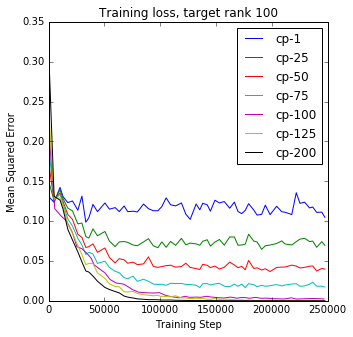
\includegraphics[width=\textwidth]{tensors/cp100cpapprox}
	\caption{Attempting to approximate by directly learning factor matrices representing a 
		CP-decomposition of various ranks}
	\label{fig:cpcpapprox}
\end{subfigure}
~
\begin{subfigure}[t]{0.45\textwidth}
	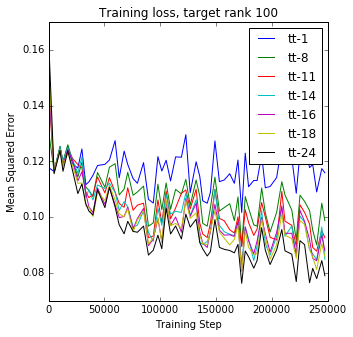
\includegraphics[width=\textwidth]{tensors/cp100ttapprox}
	\caption{Attempting to approximate by directly learning a TT-decomposition of various ranks}
	\label{fig:cpttapprox}
\end{subfigure}
\caption{Results for learning direct approximations of a CP-rank 100 tensor.}
 \label{fig:cpapprox}
\end{figure}

\begin{figure}
\centering
\begin{subfigure}[t]{0.45\textwidth}
	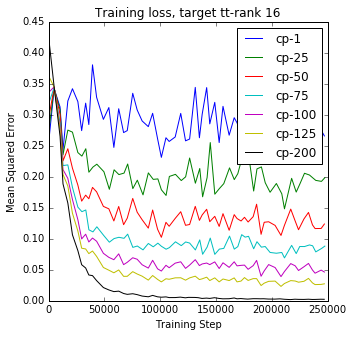
\includegraphics[width=\textwidth]{tensors/tt16cpapprox}
	\caption{Attempting to approximate by directly learning a 
		CP-decomposition of various ranks}
	\label{fig:ttcpapprox}
\end{subfigure}
~
\begin{subfigure}[t]{0.45\textwidth}
	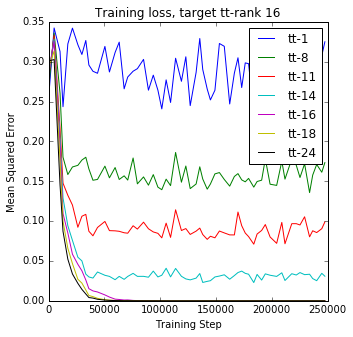
\includegraphics[width=\textwidth]{tensors/tt16ttapprox}
	\caption{Attempting to approximate by directly learning a TT-decomposition of various ranks}
	\label{fig:ttttapprox}
\end{subfigure}
\caption{Results for learning direct approximations of a tt-rank 16 tensor.}
\label{fig:ttapprox}
\end{figure}

\subsection{Learning to multiply}
\subsubsection{Goal}
Learning bilinear functions provides a way to linearly approximate functions of two variables.
A motivating example of such a function is element-wise multiplication, also known as the Hadamard
product. In this section we investigate briefly the ability of the two decompositions to model
such a product. We are particularly concerned with this as generalising this operation provides
significant motivation for the current investigation.


\subsubsection{Experiment Details}
Learning exact element-wise products is a special case and can clearly be done with the 
CP-decomposition without sacrificing parameter reduction. The question that remains is how closely
a given decomposition can approximate an element-wise product, especially if there is some kind of
helpful latent structure in the inputs to exploit. We test this by inducing a random structure
on the inputs.

This is performed identically to the experiments in section~\ref{sec:randbilin}
except that that rather than generating a random tensor to provide the targets for training,
we simply multiply element-wise the input vectors. We also simplify slightly by drawing the
input vectors from \(\{0,1\}\) with equal probability
(element-wise multiply in this sense corresponds to a bitwise AND). 
Again the squared error loss is used, although
a momentum term (with coefficient 0.9) was found to greatly assist learning.
For a further test, the target
output has a fixed permutation applied which removes the diagonal structure from the target but
should still be a straightforward task. For this task we would
expect that the CP-decomposition drastically outperforms the TT-decomposition.

For a more realistic test we introduce a random structure to the input vectors. This is done by
creating smaller vectors and expanding them to the appropriate size by copying the
elements to random positions. The mapping of positions is fixed for the duration of a training
run. We then experiment with varying the size of these smaller vectors and hence varying the
degree of correlation while keeping the rank of the decomposition fixed. Here we have fewer
preconceptions regarding the relative performance of the decompositions.

\subsubsection{Results}
The results, figures~\ref{fig:multiply-ff} and \ref{fig:permute-multiply-ff}, affirm our
expectations. The CP-decomposition is able to consistently reduce error as rank increases
 while the TT-decomposition appears to struggle.

What is more surprising is that even when there is significant structure to the inputs, the
TT decomposition is notably worse. One hypothesis is that the CP decomposition simply represents
higher rank tensors with the same number of parameters and that this is is what allows to better
represent more complex structures. This is shown in the other results -- the rank 1 decompositions
achieve similar performance regardless of the decomposition.

\begin{figure}
	\begin{subfigure}[t]{0.45\textwidth}
		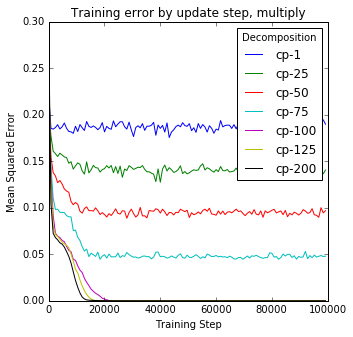
\includegraphics[width=\textwidth]{tensors/multiply-cp-mom}
		\caption{Learning curves for CP-decompositions learning element-wise multiplication}
	\end{subfigure}
	~
	\begin{subfigure}[t]{0.45\textwidth}
		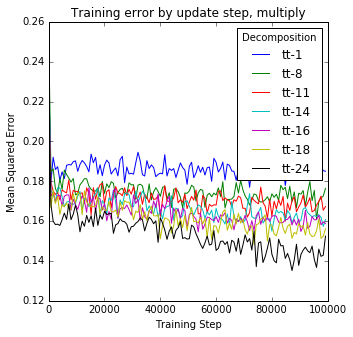
\includegraphics[width=\textwidth]{tensors/multiply-tt-mom}
		\caption{Learning curves for TT-decompositions learning element-wise multiplication}
	\end{subfigure}
	\caption{Training error for various rank decompositions on the element-wise multiplication
	task.}
	\label{fig:multiply-ff}
\end{figure}

\begin{figure}
	\begin{subfigure}[t]{0.45\textwidth}
		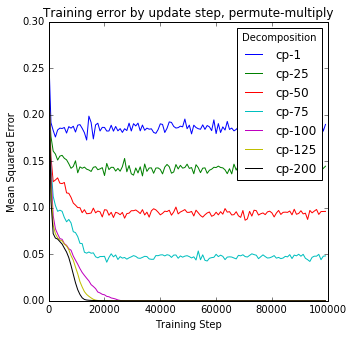
\includegraphics[width=\textwidth]{tensors/permute-cp-mom}
		\caption{Learning curves for CP-decompositions learning permuted 
		element-wise multiplication}
	\end{subfigure}
	~
	\begin{subfigure}[t]{0.45\textwidth}
		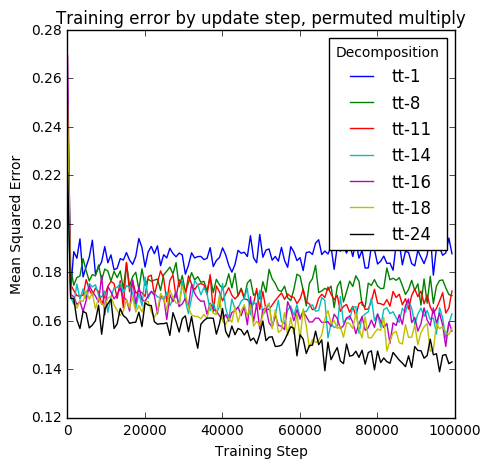
\includegraphics[width=\textwidth]{tensors/permute-tt-mom}
		\caption{Learning curves for TT-decompositions learning permuted
		 element-wise multiplication}
	\end{subfigure}
	\caption{Training error for various rank decompositions on the permuted
	element-wise multiplication
	task.}
	\label{fig:permute-multiply-ff}
\end{figure} 



The results again show the CP-decomposition outperforming the TT-decomposition dramatically.
In this case this is slightly more surprising as there is more likely to be solutions
obtainable in the TT-decomposition.


\begin{figure}
	\begin{subfigure}[t]{0.45\textwidth}
		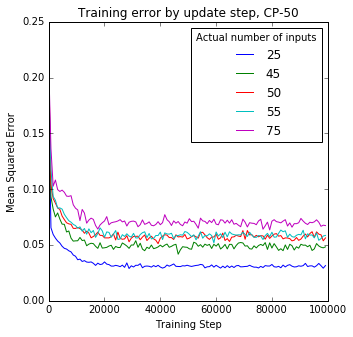
\includegraphics[width=\textwidth]{tensors/correlatecp50-mom}
		\caption{Learning curves for a rank 50 CP-decomposition.}
	\end{subfigure}
	~
	\begin{subfigure}[t]{0.45\textwidth}
		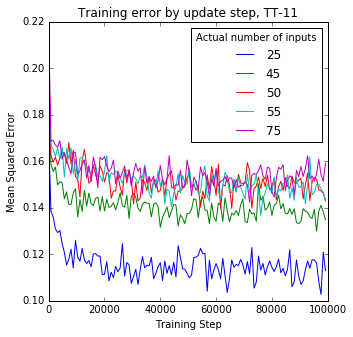
\includegraphics[width=\textwidth]{tensors/correlatett11-mom}
		\caption{Learning curves for a rank 11 TT-decomposition.}
	\end{subfigure}
	\caption{Training error for two decompositions learning element-wise multiplication with
	 varying amounts of structure.}
	\label{fig:correlate-multiply}
\end{figure}

\subsection{XOR}
\subsubsection{Goal}
Theoretical results suggest that a single tensor layer should be able to solve the exclusive-or problem.
This is known to be impossible with a single normal feed-forward layer, so if the tensor layer is successful
in this task it would provide a useful demonstration of the difference in expressive power.

\subsubsection{Experiment Details}
The truth table for exclusive-or operation can be found in table~\ref{tab:xor}. True values were represented
as \(1\) and false as \(0\). As there are only four data points, all were evaluated for each parameter update.
All models were trained using standard gradient descent with a learning rate of \(0.5\).

Three models were evaluated, a perceptron, a multi-layer perceptron (MLP) and a single layer tensor. All
models used a sigmoid nonlinearity on the output, the MLP had 4 hidden units also with sigmoids and the 
tensor layer used a rank \(1\) CP decomposition. Models
were trained to minimise the cross-entropy, averaged across the data points with training continuing
for \(1000\) epochs. Although not all MLPs had converged by this time, it was sufficient to see the difference
between the architectures. 

\subsubsection{Results}
The baseline cross entropy is 0.6931, corresponding to outputting
0.5 for all inputs (or guessing uniformly at random). As expected, the perceptron converges rapidly to this
point. Both the MLP and the tensor are able to solve the task, although it is interesting to note that the
tensor does so far more rapidly and reliably than the MLP. This is not surprising in light of
theorem~\ref{thm:xor} as this is precisely the kind of relationship we would expect the tensor product to
represent naturally.

\begin{figure}
\begin{floatrow}
\floatbox{table}
  {%
   \begin{tabu} to 0.3\textwidth {|X|X||X|}
	\hline
	Input 1 & Input 2 & Output \\
	\hline\hline
	T & T & F \\
	T & F & T \\
	F & T & T \\
	F & F & F \\
	\hline
	\end{tabu}%
  }
  {%
   \caption{Exclusive-or truth table}
   \label{tab:xor}%
  }
\ffigbox{%
\centering
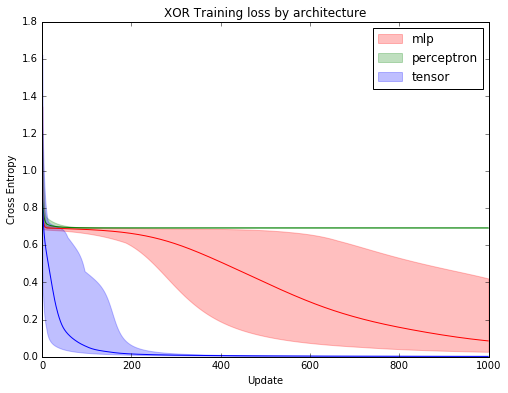
\includegraphics[width=0.45\textwidth]{tensors/xor}
}{%
 \caption[XOR results]{Exclusive-or results. Bold line is the mean of 50 runs, shading indicates the
minimum and maximum across all runs.}
}
\end{floatrow}
\end{figure}

\subsection{Separating Style and Content}
\subsubsection{Goal}
In this section we apply the tensor decompositions to a less trivial task. In particular, we
address the \textit{extrapolation} problem presented by Tenenbaum and 
Freeman. \autocite{Tenenbaum2000} The focus in this task in on data that is naturally presented as a
function of two factors, termed \textit{style} and \textit{content}. Tennenbaum and Freeman
propose the use of bilinear models for such data as follows. The aim is to verify that we
can learn a tensor decomposition of an unknown latent tensor with unknown rank.

\subsubsection{Experiment Details}
\paragraph{Problem Formulation}
Let \(\vec{y}_{sc}\) be an observation vector with style \(s\) and content \(c\). It is modelled
in bilinear form:
\begin{equation}
	\vec{y}_{sc} = \tran{\vec{a}_s}\tensor{W}\vec{b}_c
\end{equation} where \(\vec{a}_s\) and \(\vec{b}_c\) are style and content parameter vectors
respectively and \(\tensor{W}\) represents a set of basis functions independent of the parameters.
A number of tasks involving learning such a model were proposed, but we focus on extrapolation:
 learning both the parameter vectors and the basis tensor at once in such a way that
the model successfully generalises to style and content pairs not seen during training.

We model the style and content parameter vectors as fixed length, dense vectors with a unique
vector for each style label and each content label. The parameters in these vectors can be
learnt by gradient descent at jointly with the tensor \(\tensor{W}\). This is equivalent
to representing them in a one-of-N encoding (a vector with one value per possible label, all
zero apart from the entry corresponding to the label in question) and then multiplying it by
a matrix. We refer to such a matrix as an \textit{embedding matrix}. It is clear that if we
were to attempt to learn the model without these embedding matrices and simply representing
\(\vec{a}\) and \(\vec{b}\) with one-of-N encodings that the model would fail completely to
generalise. A bilinear product with two such vectors would amount to selecting a single fibre
from the tensor, so the tensor could only ever hope to directly store the training data.
Introducing a decomposition changes this by forcing the elements of the tensor to depend on
one another.


\paragraph{Data}
One dataset explored in \autocite{Tenenbaum2000} is typographical -- this provides a natural
source of data defined by two factors: font and character. We refer to the character as the
content and the font as the style. We collected a small dataset of five fonts and their
italic/oblique variants for a total of ten styles. Variation between styles comes from stroke
width, slant and the presence of absence of serifs. From each font the uppercase and lowercase
letters of the English alphabet were extracted, totalling 52 different content labels. Data was
saved as 32 pixel by 32 pixel greyscale images. To represent images as vectors for the purposes
of the above model they are flattened in scanline order: left to right and top to bottom.

\paragraph{Training Details}
This is a very difficult task as we are expecting the model to produce pictures similar to ones
that have never been seen in training. Further, we are trying to train a model with potentially
thousands of free parameters based only on a few hundred examples. As this suggests, stopping
the model from overfitting was the major challenge. The aim of the experiments was not
necessarily to achieve state-of-the-art performance, but to quickly ensure that using a tensor
decomposition to model non-trivial interactions was a feasible goal.

To begin we verify that a fairly small model is capable of representing the data. For this we
use embeddings of size \(25\) and a rank \(25\) CP-decomposition. This model has 78,350
parameters, while a model that contained the explicit \(25 \times 1024 \times 25\) tensor
would have 641,550. We train the model using ADAM \autocite{Kingma2014}, a variant of
stochastic gradient descent to minimise the squared error:
\begin{align}
	E = \sum_{i}^B ||\hat{\vec{y}}_{sc} - \vec{y}_{sc}||_2^2
\end{align} where \(B\) is the number of elements in a batch (26 was used in the following) and
\(\hat{\vec{y}}_{sc} = \vec{a}_s^\mathsf{T}\tensor{W}\vec{b}_c\) is the predicted image. Both
the central tensor and the embedding vectors are updated at every update step. A small amount
of \(l_2\) regularisation was found to help prevent overfitting, this involves adding a penalty
term to the loss of the form \(\lambda||\mat{X}||_F^2 = \lambda\sum_i^m\sum_j^mX_{ij}^2\) for
each matrix in the model.

\subsubsection{Results}
Figure~\ref{fig:sandc-interp} provides a visual inspection of what the model was able to
learn. Images were generated by finding the style and content labels for a two examples and
linearly interpolating first the content vector and then the style vector, generating an
image with the intermediate vectors at each step. 

The start and end images are not perfect; the model was small and unable to capture the training
data exactly. During experimentation larger models were found to fit the data very well, but 
overfitted rapidly, which is why a smaller model was used for these results.

Intermediate stages of the interpolation have no real meaning but they indicate that the model has
not simply learned to recall individual pairs of labels. We see that as either the content or
the style shifts from one to another, the elements of the source image which are not shared with
the target fade out and are replaced.

Results on unseen data are shown in figure~\ref{fig:sandc-valid}. These show that the model does
appear to capture some of the salient information for separating the style and content. In
particular, the general shapes of the letters are roughly appropriate and it has begun to capture
some information about the presence or absence of serifs and general slant.
Figure~\ref{fig:sandc-fail} shows a harder example -- the lowercase `a' has considerable variation
among various fonts and the model is unable to guess what would be appropriate for an unseen
example. 

Overall, these results show the tensor was capable of learning a model for the data.
This suggests that the aim of inserting such tensor products into more complex neural networks
is feasible, reinforcing the promising theoretical results.


\begin{figure}
	\begin{subfigure}[t]{\textwidth}
	\begin{tabu} to \textwidth {XXXXXXXXXX}
		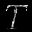
\includegraphics[width=0.09\textwidth]{tensors/sandc/interp/output0} &
		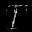
\includegraphics[width=0.09\textwidth]{tensors/sandc/interp/output1} &
		
\includegraphics[width=0.09\textwidth]{tensors/sandc/interp/output2} &
		
\includegraphics[width=0.09\textwidth]{tensors/sandc/interp/output3} &
		
\includegraphics[width=0.09\textwidth]{tensors/sandc/interp/output4} &
		
\includegraphics[width=0.09\textwidth]{tensors/sandc/interp/output5} &
		
\includegraphics[width=0.09\textwidth]{tensors/sandc/interp/output6} &
		
\includegraphics[width=0.09\textwidth]{tensors/sandc/interp/output7} &
		
\includegraphics[width=0.09\textwidth]{tensors/sandc/interp/output8} &
		
\includegraphics[width=0.09\textwidth]{tensors/sandc/interp/output9} 
	\end{tabu}
	\caption{Linearly interpolating between two content vectors (`T' to `m') with style vector
			 fixed.}
	\end{subfigure}
	
	\begin{subfigure}[t]{\textwidth}
	\begin{tabu} to \textwidth {XXXXXXXXXX}
		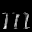
\includegraphics[width=0.09\textwidth]{tensors/sandc/interp/output10} &
		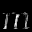
\includegraphics[width=0.09\textwidth]{tensors/sandc/interp/output11} &
		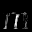
\includegraphics[width=0.09\textwidth]{tensors/sandc/interp/output12} &
		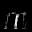
\includegraphics[width=0.09\textwidth]{tensors/sandc/interp/output13} &
		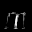
\includegraphics[width=0.09\textwidth]{tensors/sandc/interp/output14} &
		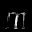
\includegraphics[width=0.09\textwidth]{tensors/sandc/interp/output15} &
		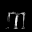
\includegraphics[width=0.09\textwidth]{tensors/sandc/interp/output16} &
		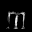
\includegraphics[width=0.09\textwidth]{tensors/sandc/interp/output17} &
		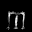
\includegraphics[width=0.09\textwidth]{tensors/sandc/interp/output18} &
		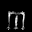
\includegraphics[width=0.09\textwidth]{tensors/sandc/interp/output19}
	\end{tabu}
	\caption{Linearly interpolating between two style vectors with fixed content.}
	\end{subfigure}
	\caption{Learned style and content representations.}
	\label{fig:sandc-interp}
\end{figure}

\begin{figure}
	\begin{subfigure}[t]{\textwidth}
		\begin{tabu} to \textwidth {XXXXXXXXX}
			
\includegraphics[scale=1]{tensors/sandc/valid/real/Georgia-76} &
			
\includegraphics[scale=1]{tensors/sandc/valid/real/Georgia-77} &
			
\includegraphics[scale=1]{tensors/sandc/valid/real/Georgia-83} &
			
\includegraphics[scale=1]{tensors/sandc/valid/real/VeraMoIt-86} &
			
\includegraphics[scale=1]{tensors/sandc/valid/real/VeraMoIt-100} &
			
\includegraphics[scale=1]{tensors/sandc/valid/real/VeraMoIt-101} &
			
\includegraphics[scale=1]{tensors/sandc/valid/real/VeraMono-66} &
			
\includegraphics[scale=1]{tensors/sandc/valid/real/VeraMono-76} &
			
\includegraphics[scale=1]{tensors/sandc/valid/real/VeraMono-89} 
		\end{tabu}
		\caption{Actual images from the dataset.}
	\end{subfigure}
	
	\begin{subfigure}[t]{\textwidth}
		\begin{tabu} to \textwidth {XXXXXXXXX}
			
\includegraphics[scale=1]{tensors/sandc/valid/synth/Georgia-76} &
			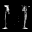
\includegraphics[scale=1]{tensors/sandc/valid/synth/Georgia-77} &
			
\includegraphics[scale=1]{tensors/sandc/valid/synth/Georgia-83} &
			
\includegraphics[scale=1]{tensors/sandc/valid/synth/VeraMoIt-86} &
			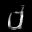
\includegraphics[scale=1]{tensors/sandc/valid/synth/VeraMoIt-100} &
			
\includegraphics[scale=1]{tensors/sandc/valid/synth/VeraMoIt-101} &
			
\includegraphics[scale=1]{tensors/sandc/valid/synth/VeraMono-66} &
			
\includegraphics[scale=1]{tensors/sandc/valid/synth/VeraMono-76} &
			
\includegraphics[scale=1]{tensors/sandc/valid/synth/VeraMono-89} 
		\end{tabu}
		\caption{Model output, having never seen these specific pairs during training.}
	\end{subfigure}
\caption{Example of images generated from unseen style and content pairs, three letters from
		 three different fonts.}
\label{fig:sandc-valid}
\end{figure}


\begin{figure}
	\begin{center}
	\begin{subfigure}[t]{0.45\textwidth}
		\centering
		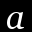
\includegraphics[scale=1]{tensors/sandc/valid/real/Georgiai-97}
		\caption{From the data}
	\end{subfigure}
	~
	\begin{subfigure}[t]{0.45\textwidth}
		\centering
		\includegraphics[scale=1]{tensors/sandc/valid/synth/Georgiai-97}
		\caption{Generated}
	\end{subfigure}
	\end{center}
	\caption{A difficult example.}
	\label{fig:sandc-fail}
\end{figure}


